\chapter{Methodology}

Our processing pipeline uses a combination of open source software for research purposes (MedInria) and developed in our lab for our very specific needs of reproducible experiments \cite{piuzephd}. As explained in the previous section the first step is to use MedInria to read the DICOMs and get the tensor matrix presented in Section \ref{diffusion_tensor_matrix} at every voxel, as well as the FA and ADC in reusable Matlab file format.

In this chapter we will explain how Cartan frames and the approximations of the 1-forms are an appropriate fit for the data that we have. This will be illustrated by some examples from our dataset. The detailed experimental results on the pig hearts along with the discussion of those results will be presented in Chapter 4.

\section{Rician noise smoothing}

We used an established Rician smoothing method to deal with noise in the diffusion images \cite{wiest2008rician}. This is a type of non-local smoothing technique which uses voxel to voxel similarity to guide the smoothing process. In general the parameters for this filtering method must be tuned to prevent oversmoothing, which can happen for instance if the weight is not sufficiently penalized when the similarity is not high enough. This was the very first step of our data processing pipeline.

\section{Getting fiber directions from the diffusion tensor matrix}

Once we have our diffusion tensor matrix $\mathbb{D}$, a simple eigenvector and eigenvalue calculation gives us the eigenvalues $(\lambda_1, \lambda_2, \lambda_3)$ and the corresponding eigenvectors $(\nu_1, \nu_2, \nu_3)$.
\begin{align}
    \mathbb{D} &= \begin{pmatrix}
        D_{xx} & D_{xy} & D_{xz} \\
        D_{yx} & D_{yy} & D_{yz} \\
        D_{zx} & D_{zy} & D_{zz}
        \end{pmatrix} \\
    &= \mathbb{P}^{-1} \mathbb{\tilde{D}P}
\end{align}
where:
\begin{gather*}
    \mathbb{\tilde{D}} = \begin{pmatrix}
        \lambda_1 & 0 & 0 \\
        0 & \lambda_2 & 0 \\
        0 & 0 & \lambda_3
        \end{pmatrix} \\
    \mathbb{\tilde{D}}\cdot \nu_1 = \lambda_1 \nu_1 \\
    \mathbb{\tilde{D}}\cdot \nu_2 = \lambda_2 \nu_2 \\
    \mathbb{\tilde{D}}\cdot \nu_3 = \lambda_3 \nu_3
\end{gather*}
The biggest eigenvalue in absolute value will correspond to the fiber direction and sorting those will give us the eigenvector corresponding to the fiber direction. We can also at this point get the FA and ADC values to double check what MedInria gave us.\\
All the eigenvectors at every voxel we obtain from this process do not always point in the same direction, and sometimes neighbor voxels will have fibers pointing in opposite direction. To solve this issue, a cylindrical consistency processing step was applied \cite{pami2015}. The idea is to compute from the mask of the heart studied a gradient pointing at each voxel from the inner wall to the outer wall. Once this gradient is obtained, this preprocessing step ensures that all cross products of the eigenvectors and the gradient are of the same sign. If not, then we just change the sign of the eigenvector.

\section{Modeling fiber geometry using connection forms}

Connection forms measure the local rotations of the frame axes $\mathbf{f}_1, \mathbf{f}_2, \mathbf{f}_3$. Here we focus on the contraction of the 1-form $c_{12}$ on the frame axes $\mathbf{f}_3$ and compare its values in a short axis slice of a pig heart with an infarct - Fig. \ref{fig:c123infarcted} - with those in a short axis slice from a healthy pig heart - Fig. \ref{fig:c123healthy}.
\begin{figure}[h!]
    \centering
    \begin{subfigure}[h!]{0.48\textwidth}
        \centering
        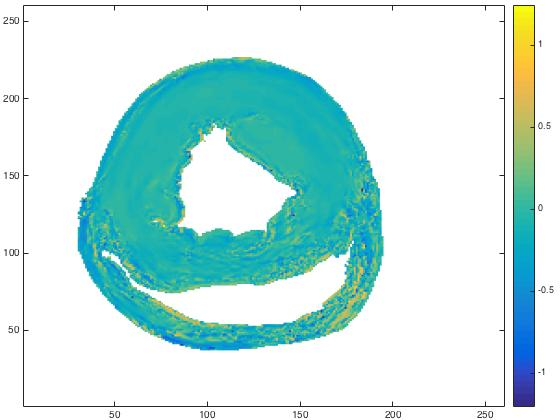
\includegraphics[width=\textwidth]{figures/pig4_c123_slice_19}
        \caption{$c_{123}$ (infarcted)}
        \label{fig:c123infarcted}
    \end{subfigure}
    \hfill
    \begin{subfigure}[h!]{0.48\textwidth}
        \centering
        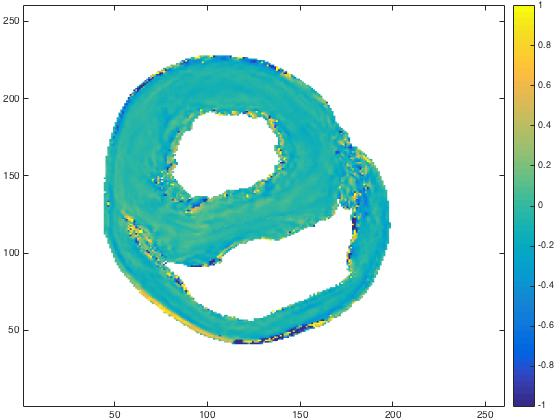
\includegraphics[width=\textwidth]{figures/pig25_c123_slice_30}
        \caption{$c_{123}$ (healthy)}
        \label{fig:c123healthy}
    \end{subfigure}
    \caption{$c_{123}$ with range of values in porcine hearts}
    \label{fig:c123all}
\end{figure}

In a qualitative sense, observing the colormap and comparing the smoothness of figures \ref{fig:c123infarcted} to the control heart in Fig. \ref{fig:c123healthy}, we can already notice how in the healthy case and in regions remote from the infarct in the infarcted case we have smooth and regular colors which represent a rather constant value of $c_{123}$. On the other hand, in the infarct region it is clear that the values vary a lot more and give a strong impression of a lack of coherence. A more quantitative approach will be discussed in Section \ref{histogram_section}.
\begin{figure}
    \centering
    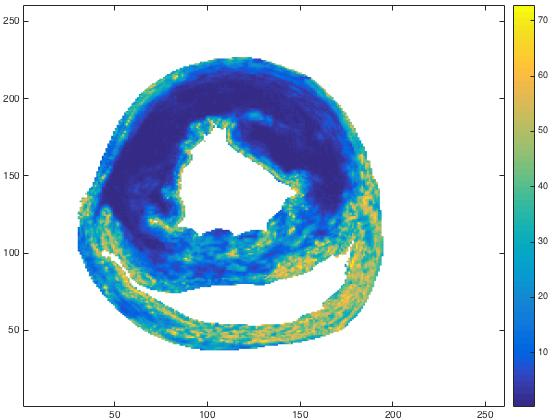
\includegraphics[width=\textwidth]{figures/pig4_error_of_fit_slice_19}
    \caption{Error of fit, giving the absolute angle difference between our estimation from the connection forms and the ground truth}
    \label{fig:error_of_fit}
\end{figure}
 
Cartan frame field analysis applies to smoothly rotating frame fields. In the presence of infarcts fiber orientation coherence is lost. The connections then fail to explain the orientation of fibers in a local neighborhood and fitting errors using this method go up as we can observe in Fig. \ref{fig:error_of_fit}. This association of frame field fitting error with fiber incoherence is the key insight behind the developments in this thesis.

\section{Cartan Frame Fitting and Error Analysis}

As explained earlier, at each voxel we use an estimate of the fiber orientation given by the orientation of the first principal eigenvector of a diffusion tensor reconstruction for $\mathbf{f}_1$. We then estimate the heart wall normal as the gradient of the distance function to the boundary of the myocardium and take the component of the normal that is orthogonal to $\mathbf{f}_1$ to be $\mathbf{f}_3$. $\mathbf{f}_2$ is then taken to be their cross product. Our numerical implementation of frame field fitting relies on finding the best estimates of the 9 connection forms at each voxel in the sense of explaining the orientations in its neighborhood. Specifically, using Nelder-Mead optimization, we minimize an energy given by the angle between the measured orientation at each neighbor and that given by rotating the frame field by a particular set of connections, explained in Section \ref{fitting_method}. Once this method converges the error of fit at a voxel is taken to be the average angular error between fiber orientations in a neighborhood and those given by rotating the frame at that voxel using its connection parameters.